\chapter{Parallelization and Scaling}
\label{chap:Parallelization and Scaling}

We find the ability to utilize available hardware important when designing a high performance system for OLAP workloads. For maximal performance, a system must be parallelized on all levels:

\begin{enumerate}
  \item Utilize computing power in a distributed, share-nothing environment.
  \item Utilize all sockets in a non-uniform memory access (NUMA) architecture.
  \item Exploit thread-level parallelism within a multicore processor.
  \item Exploit instruction level parallelism within a single core.
  \item Use single input, multiple data (SIMD) instructions available in the processors.
\end{enumerate}

One of the keys to acheiving good parallel performance, is to use structures that are built for distributed and multi-core environments \cite{Primsch2011-ij}. \exasol, the top performing system on the TPC-H benchmark, applies parallelism on every layer \cite{Exasol2014-xh}.

\newpage

\section{Parallelism in a Distributed, Shared-Nothing Architecture}
\label{sec:Parallelism in a Distributed, Shared-Nothing Architecture}
For performance reasons, a database may be distributed across multiple servers. We refer to this as a \textit{shared-nothing} architecture, as all communication between the servers in the cluster must explicitly be passed through the network \cite{DeWitt1992-ki}. Operations are performed locally on each server, and only refined and processed data is sent back to the client program. This reduces network traffic and keeps the system scalable.


%Scaling out is the technique where several machines (nodes) are used, and the work is distributed between them. They share no common resources, so all data and control traffic must be passed through explicit network actions. This technique can be used to support (i) more users, (ii) more data, and (iii) improve performance.

Several of the systems studied in this research supports a distributed architecture. Among them are \oracle~\cite{Mukherjee2015-ul}, \cstore~\cite{Stonebraker2005-qz}, \saph~\cite{Farber2012-vh} and \exasol~\cite{Exasol2014-xh}. These systems are distributed in terms of intra-query parallelism, that is each query are may be executed on all servers.

\afigure{img/oracle-distributed.png}{\oracle~in-memory compression units (IMCUs) distributed across different nodes in a shared nothing architecture. Courtesy of \cite{Mukherjee2015-ul}.}{fig:oracle-distributed}{0.7}
In Section \ref{sec:Horizontal Partitioning}, we saw that \oracle~horizontally partitions the columns into in-memory compression units (IMCUs). In a distributed environment, these IMCUs can be spread across different nodes \cite{Mukherjee2015-ul}, as seen in Figure \ref{fig:oracle-distributed}. The blocks is be distributed using a two-phase strategy. First, a centralized coordination phase is performed such that servers can a minimal consensus can be established. Second, IMCUs are spread in a decentralized manner. \oracle~in a distributed environment can be configured to be both \term{1-safe}and \textit{(N-1)-safe}.


\qlikview~too supports a distributed architecture, but more in terms of supporting more users, which we will look into closer in the section about scaling (Section \ref{sec:Scaling}). Using different load balancing strategies, like random, and loaded document, more users are supported \cite{Qlik2012-ku}. However, each application application cannot be spread across multiple servers, an entire copy must be kept per server \todo{find out more about this}. 

\subsection{Distributed Dictionary}
\label{sub:Distributed Dictionary}
\ffigure{img/dictionary-scale-out}{Different data placements of a dictionary encoded column with an inverted index. Courtesy of \cite{Psaroudakis2015-lc}.}{fig:dictionary-scale-out}
In a shared-nothing architecture, the column can be spread out in three different ways, as seen in Figure \ref{fig:dictionary-scale-out}. When using dictionary compression, there are several ways to spread the dictionaries across the partition \cite{Psaroudakis2015-lc}. Physical partitioning, as used by for instance \oracle~has the disadvantage of reducing compression rates. The various schemes has a time to build versus performance trade-off. \todo{Elaborate and explain the figure more}.

\paragraph{Round-robin (RR)}
\label{par:Round-robin (RR)}
Each node in the cluster get a column each. Here, compression is maximized, but it does not account for data skew and certain columns might be hot-spots.

\paragraph{Index-Vector Partitioned (IVP)}
\label{par:Index-Vector Partitioned (IVP)}
This keeps a maximum compression for the dictionary, and values are spread evenly accross all data nodes. However, this structure is hard to construct and maintain. Lastly, this technique requires inverted indexes on the dictionary, a structure we have recommended against in Chapter \ref{chap:Indexes and Auxiliary Structures}.

\paragraph{Physically Partitioned (PP)}
\label{par:Physically Partitioned (PP)}
Here, the columns are split, and for each column partition, a dictionary is constructed. This technique minimizes compression (as dictionary entries might be duplicated per block) and certain operations might be more tedious to implement. 

\section{Thread-level parallelism}
\label{sec:Intra-query Parallelism and Scheduling}
% paragraph introducing the "problem"
Within a single multiprocessor, where all processing units share memory, parallelization can be performed by using threads. Ideally, queries should use all available resources, and if a query is run one by one, the ultimate goal is that a query speeds up linearly with the number of processing units available. In a database system, Parallelization is normally solved by partitioning the input onto the available processing units and merge the results after computation is done \cite{Neumann2011-uq}.

% paragraph of which systems using parallelism
Most modern database management systems use thread-level parallelism to improve performance. Systems here include \vertica~\cite{Lamb2012-kg}, \mssql~\cite{Larson2013-mc}, \blink~\cite{Barber2012-xt, Johnson2008-cp}, \saph~\cite{Farber2012-vh}. \exasol, the top performing system on the TPC-H benchmark, reports to apply \textbf{parallelism on every layer} \cite{Exasol2014-xh}. As for reference products in our research, \qlikview~has reported that it scales almost perfectly with the addition of more cores \cite{Qlik2011-ef}.

% paragraph explaining how each system splits queries
In terms of work distribution, \blink~parallelized on a block level, where each partition is split into blocks and assigned to a thread \cite{Johnson2008-cp, Barber2012-xt}. \mssql~divides the query into batches, and the batches are consumed and processed by all the threads in the system \cite{Larson2013-mc}. One execution model is the task-based query execution model which is used by \hyrise~\cite{Swhalb2014-hn}. They claim almost perfect load balancing on multi-core CPUs, and it has efficient workload management.

% paragraphs illustrating the main challenges with parallelization and techniques used to fix it
The barriers for linear speedup is startup costs, interference and communication, and unevendistribution of work (data skew)\cite{DeWitt1992-ki}, which translates to that the key challenges in query processing is work distribution and scheduling \cite{Neumann2011-uq}. In addition, parallel joining and grouping/aggregation is not trivial to do in parallel. We study this in Section \ref{sub:Parallel Joining} and Section \ref{sub:Parallel Grouping and Aggregation} respectively.

\subsection{Scheduling}
\label{sub:Scheduling}
Getting scheduling right is a hard process \cite{Psaroudakis2013-fn}. First of all, all scheduling cannot be given to the operating system due to high creation costs and context switches. Secondly, all available threads for a node should be in one single thread pool. \oracle~uses three thread pools (dispatchers, executors, and receivers), but these are oblivious to each other and hurt performance. One of the main problems addressed in this paper is that queries divides into a number of tasks irrespective of how many other concurrent tasks that are running. That is, if the CPU is processing on six out of eigth cores, only two threads should be spawned for a query.

\ffigure{img/scheduler.png}{Data structures used by a task scheduler. Courtesy of \cite{Psaroudakis2013-fn}.}{fig:scheduler}
A typical query can be represented as a directed acyclic graph (DAG), where each node is a separate task. Each thread can pick any task from the DAGs where the predecessor has already been processed. The throughput/latency tradeoff can be adjusted by changing the probability that a root node (new query) is selected. The structures used by the scheduler is depicted in Figure \ref{fig:scheduler}.

Conclusion: One single thread pool. Queries should calculate the number of tasks based on how many threads that are already running.

Performance can be boosted if tasks are allowed to be stolen from other work units. This is done in \blink~\cite{Barber2012-xt}. However, special attention should be given to which tasks that are stolen. Ideally, one should only steal computing intensive tasks, not memory intensive ones \cite{Psaroudakis2015-lc}.


\subsection{NUMA awareness}
\label{sub:NUMA awareness}
\afigure{img/numa.png}{4-socket server with Ivybridge-EX CPU. Each socket has its own caches, an transfering data between sockets takes longer time than accessing data local to a socket. Courtesy of \cite{Psaroudakis2015-lc}}{fig:numa}{0.7}
We saw in the background section that non-uniform memory access (NUMA) machines are machines where different parts of memory have different access time. Memory in these machines are decentralized, so communication costs must be taken account for among sockets \cite{Psaroudakis2015-lc}. On such machines, the database system should be aware of this to make better scheduling decisions. A NUMA aware system can have up to 5x performance compared to a system which is not \cite{Psaroudakis2015-lc}. \todo{QlikView2011-yc also has some background on NUMA}

An example of such system is \hyper~\cite{Psaroudakis2014-ma, Psaroudakis2015-lc}. \hyper distributes works across socekts, uses task stealing and elastic parallelism. Data locality is optimized. In this system, tasks are divided into two classes: Memory intensive and CPU intensive. Memory intensive tasks should not be stolen across sockets, but this is OK for CPU intensive tasks.

The \qlikview~developers conclude that NUMA is great if the application can take advantage of it, but if not, NUMA might have a negative impact \cite{Qlik2013-an}. By turning off NUMA, either through a soft switch in the program, or in the node's BIOS, \qlikview~performs better.

Lastly, utilizing techniques for distributed, shared-nothing architectures might enhance performance on NUMA nodes \cite{Mukherjee2015-ul}. By treating each socket as a single server instance, and let all communication be performed with explicit message passing, performance might be improved.

Psaroudakis \ea~suggest using a page socket mapping structure for keeping track which processor owns which partition \cite{Psaroudakis2015-lc}.

\subsection{Hyperthreading}
\label{sub:Hyperthreading}
Hyper-threading is a technique used in most modern processors where each core has two logical cores per actual core. It is mainly used as a technique to reduce the memory-gap. Hyperthreading will for instance speed up the probe phase in joins \cite{Barber2014-ey}.

However, if a thread never waiting for memory, hyperthreading will degrade performance. \qlikview~whitepaper say that hyperthreading should be disabled for maximum performance \cite{QlikView2011-yc}. 

\section{Instruction Level Paralellism}
\label{sec:Instruction Level Paralellism}
Due to super-scalar CPUs, one might optimize for instruction level paralellism. This is exploited by \blink, where query execution is executed in batches on multiple rows at the same time \cite{Johnson2008-cp}. In general, the idea is that if a processor can find enough independet work, it can be a magintude or two faster \cite{Boncz2005-wj}.\todo{Insert something here about DIRA?}

\section{Single Input, Multiple Data (SIMD)}
\label{sec:Single Input, Multiple Instructions (SIMD)}
\ffigure{img/simd.png}{SIMD execution model: In (a) scalar mode: one operation produces one result. In (b) SIMD mode: one operation produces multiple results. Courtesy of \cite{Willhalm2009-hu}.}{fig:simd}
% Present problem
Within a single thread, it instructions working on more than one element at a time can be used to enhance query performance. It is a good idea, especially if we can keep the whole block in the registers \cite{Neumann2011-uq}. An example SIMD instruction is depicted in Figure \ref{fig:simd}.


This is used by \oracle~\cite{Lahiri2015-mz}, \blink~\cite{Barber2012-xt}, \ibm~\cite{Raman2013-em}. \exasol~also reports uning SIMD instructions in query execution.

Many ALUs does not support long words, like the Intel SSE and Intel AVX2 extension \cite{Willhalm2009-hu, Willhalm2013-rl}. The key is to pack columns densely and work on multiple rows or columns at a time \cite{Johnson2008-cp}. SIMD instructions can evaluate equal-value and value-range predicates without the need of decompression.

Several compression techniques benefits from SIMD \cite{Lemke2010-is}. This is especially the case for dictionary compression.

Although algorithms can be optimized for scalar execution, the research of Willhalm \ea~show that a vectorized model is 1.58 times faster than query processing optimized for scalar execution \cite{Willhalm2009-hu}. In addition, byte aligned columns perform the best.

The highest performing database on the TPC-H benchmark uses SIMD instructions \cite{Exasol2014-xh}.

All predicates are run in parallel in \blink~\cite{Raman2008-gi} with no branching or short-circuiting.

\subsection{Aligning Words for SIMD Execution}
\label{sub:Aligning words for SIMD execution}
\begin{figure}
  \centering
  \begin{subfigure}{0.45\textwidth}
    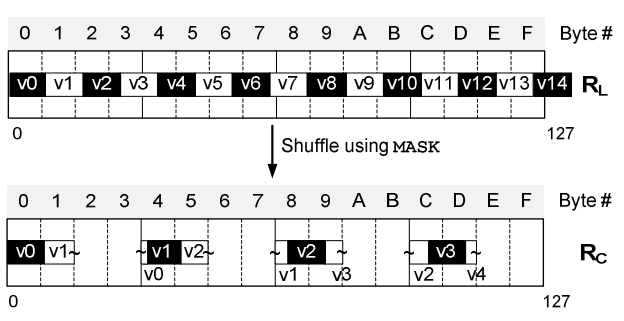
\includegraphics[width=\textwidth]{img/simd-align-1.png}
    \caption{...}
    \label{fig:simd-align-1} 
  \end{subfigure}
  \begin{subfigure}{0.45\textwidth}
    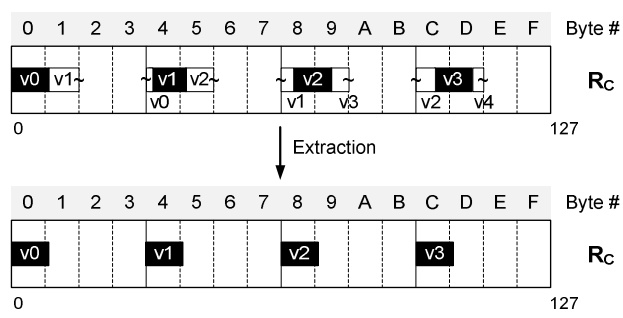
\includegraphics[width=\textwidth]{img/simd-align-2.png}
    \caption{...}
    \label{fig:simd-align-2} 
  \end{subfigure}
  \caption{Aligning a bitpacked vector for SIMD execution. Courtesy of \cite{Willhalm2009-hu}.}
  \label{fig:simd-align} 
\end{figure}
In order to use SIMD instructions, words must be aligned for the execution \cite{Willhalm2009-hu}, as seen in Figure \ref{fig:simd-align}.

Using its row-bank layout, \blink~has does not require aligning data in a word \cite{Johnson2008-cp}. For each partition, a special bitmap can be created to query the column. One or a couple of bitmap operations on every column, and then checking for null, predicates can be evaluated in a \textit{SIMD like fashion}.


\section{Scaling}
\label{sec:Scaling}
Scaling is necessary in large businesses, and volumes are increasing \cite{Qlik2012-ku}.

A system that supports this architecture can be scaled by adding more servers to the system cluster. We refer to this type of scaling as \textit{scaling out}. A system can also be scaled by adding more hardware, like more cores, more RAM, more powerful processors etc. to a single server. We refer to this type of scaling as \textit{scaling up}.

The best discussion on the need for scaling out can be found in research executed by Mukherjee \ea~\cite{Mukherjee2015-ul}. Historically, it has been argued that scaling out is the best way to acheive good performance. It does also provide redundancy; if one node in the cluster goes down, another node can be ready to take over.

However, there has been discussions that one should scale up instead of scale out. Wwhen using a shared-memory apporach, scaling up has been claimed to be easier \cite{Boncz2002-yj}. In addition, 80\% of Facebooks tasks is less than 10GB, a workload where a single server is sufficient \cite{Mukherjee2015-ul}. However, scaling up might also mean the transition to NUMA nodes, and these nodes (as we see in Section ?) benefit from software written for a distributed architecture. Last, but not least, if results are cached and used by several users, having one powerful server instead of several less powerful will increase cache hit rates \cite{qlik2012-ku}. \qlikview has reported that scaling up is twice as fast as scaling out on a large application with many users. For smaller applications, scaling up and scaling out gives the same performance.

Although \qlikview \cite{Qlik2012-ku} allows "proper" scaling out, that is distributing the work across multiple servers, single applications and data extracts can be spread across different servers. \todo{Elaborate and explain}



\section{Other}
\label{sec:Other}
Concurrency can be limited by having a maximum limit of concurrent queries. This is used in \ibm~\cite{Raman2013-em}.

None of this system investigated in this research have used the GPU for query processing. The reason for this might be because the GPU has bandwidth limitations \cite{Willhalm2009-hu} \todo{fill in}

The most trivial way to achieve better throughput is to allow multiple querys run at once. We refer to this technique as \textit{inter-query parallelism}.

For this to work well, query execution must be free for of locks, which is normally the case for read-only queries.

\section{Chapter Conclusion}
\label{sec:Chapter Conclusion}
We suggest using parallelization to utilize available CPU. 

We do not reccomend looking at scale-out yet, as this is harder to implement and degrades database cache performance. Instead, we recommend two scaling techniques:
\begin{itemize}
  \item Scale-out through spreading \bd~applications and data extracts across different servers.
  \item Scale-up by provisioning powerful, multicore CPUs and plenty of RAM.
\end{itemize}
